\newcount\Comments  
\Comments=1   
\documentclass[a4paper,12pt, english]{article}
\usepackage[top=2cm, bottom=2cm, left=2cm, right=2cm]{geometry}

\usepackage{babel}
\usepackage{subfigure}

\usepackage{color}

\definecolor{darkgreen}{rgb}{0,0.5,0}
\definecolor{purple}{rgb}{1,0,1}
\usepackage{graphicx}

\newcommand{\kibitz}[2]{\ifnum\Comments=1\textcolor{#1}{#2}\fi}
% add yourself here:
\newcommand{\ls}[1]{\kibitz{red}      {[Larisa: #1]}}
\newcommand{\cg}[1]  {\kibitz{purple}   {[Crina: #1]}}
\newcommand{\ns}[1]{\kibitz{cyan}     {[Noureddin: #1]}}



\usepackage{listings}
\usepackage{url}
%\usepackage{graphicx}

\usepackage{verbatim}

%\usepackage{caption}
%\usepackage{datetime}

%\onehalfspacing

\begin{document}

\title{Transfer Learning Experiment}
%\date{Mar 2014}
%\author{By: Noureddin Sadawi}
%\maketitle

%\large
\section{Scenario}
Let us assume that we have a \textbf{small} labeled dataset from one domain (we are going to call this dataset the $Target Dataset$) and [usually] it is costly to obtain new labelled data from the same domain (so the quantity is limited). \\

Also, let us also assume that we have one or more \textbf{large} and labeled datasets from a \textbf{\emph{related}} domains (we are going to call these datasets the $Source Datasets$) and [usually] it is affordable to obtain new labelled data from these domains.\\

%In classification learning, it is usually assumed that training and test sets have identical distributions!\\

If we would like to build a model for the $Target Dataset$ using it alone, then the model will likely perform undesirably as the dataset is quite small!\\

The idea is to make maximum use of the $Source Datasets$  to build a model for the $Target Dataset$ and classify data from its domain. In other words, we want to reuse data from the source tasks to augment the target task's training data (this is Instance Transfer Learning)\\

In this experiment, I have used the technique explained in a paper called \textit{"Selective Transfer Between Learning Tasks Using Task-Based Boosting"} to gain knowledge from the $Source$ data and use it in training a classifier for the $Target$ data. The proposed algorithm is called $TransferBoost$ and it is based on the classical $AdaBoost$ Algorithm!\\

\section{How TransferBoost Works (from the abovementioned paper)}
As the source and target data are from different but related domains, the two tasks (i.e. source and target) have different distributions. Yet, some of the source tasks' data could have been drawn from the target task's distribution. Such data could then be used as additional training data for the target task.\\

$TransferBoost$ attempts to automatically select individual data from the source tasks to augment the target task’s training data. It automatically determines the weight to assign to each source instance in learning the target task's model, building on the $AdaBoost$ algorithm. TransferBoost iteratively constructs an ensemble of classifiers, reweighting both the source and target data via two types of boosting: individual and task-based.\\
It increases the weight of individual mispredicted instances following AdaBoost. In parallel, it also performs task-based boosting by reweighting all instances from each source task based on their aggregate transfer to the target task.\\

In effect, TransferBoost increases the weight of source tasks that show positive transfer to the target task, and then reweights the instances within each task via AdaBoost. 

\begin{comment}
\section{How TrAdaBoost Works}
$TrAdaBoost$ is an extension of the classical $AdaBoost$ Algorithm. The technique works by voting on the usefulness of each instance of the $Source$ data (i.e. giving each instance a weight according to how close/useful it is to the $Targert$ data)\\

This learning process corresponds to transferring knowledge learned from the $source$ data to a new situation (the $target$ data) -- and this is Instance Transfer Learning.\\
\end{comment}


\section{Experiment I}
\subsection{The Data}
\begin{itemize}
\item By looking at the table provided with the Eve data, I have extracted and merged labeled data from the Sapphire Channel (Sapphire Active/Inactive) for assays TS3 and TS6. This is for strain \emph{Plasmodium vivax}. This is going to be our $Source Dataset$

\item I have also extracted labeled data from the Venus Channel (Venus Active/Inactive) for assay TS6. This is for strain \emph{Plasmodium falciparum}. This is going to be our $Target Dataset$
\item I have split the $Target Dataset$ into two subdatasets. One for training and one for testing. Notice that this training subdataset is going to be our actual $Target Dataset$
\item Now our datasets look like:
   \begin{itemize}
	\item $Source Dataset$ has 2781 instances (for Pv from TS3 and TS6 -- file TS3-TS6-Pv-Source.arff)
	\item $Target Dataset$ has 46 (for Pf from TS6 -- file TS6-Pf-Target.arff)
	\item $Test Dataset$ has 1389 (for Pf from TS6 -- file TS6-Test-Pf.arff)
   \end{itemize}  
\end{itemize}  

\subsection{Experimental Setup}
The authors of the paper have provided the java source code of their implementation so I have downloaded it, plugged it into WEKA's source code and recompiled WEKA.\\
Remember that our $Target Dataset$ is quite small and our $Source Dataset$ is large and from a related domain.\\
We will use our $Test Dataset$ for evaluation (it is from the same domain as $Target Dataset$)\\

Here is what I have done:
\begin{itemize}
\item I have built a classification model with the TransferBoost Algorithm using both the $Target$ and $Source$ Datasets to carry out Transfer Learning. I used \emph{Decision Stump} as the base classifier.
\item I have built classification models with WEKA's NaiveBayes, SVM, KNN and J48 Decision Trees using the $Target Dataset$ only. This is because usually we build models using data from the same domain!
\end{itemize}

\subsection{Column Names:}
I have abbreviated column names in the following tables to save display space. In order from left to right, they're as follows:\\
Percentage of Correct guesses,\\
Percentage of Incorrect guesses,\\
Area Under the Curve (for class Active),\\
Kappa statistic,\\
Mean Abs Error,\\
Root Mean Squared Error,\\
Relative Abs Error,\\
Root Relative Squared Error,\\
Precision (for class Active),\\
Recall (for class Active),\\
F-Measure (for class Active),\\
Error Rate\\


\subsection{Experimental Stat Results 1}
In this experiment I did 10 fold cross validation using the target dataset only (built models using the target dataset only and used it for the validation)
\begin{small}
\begin{center}
    \begin{tabular}{ | l | l | l | l | l | l | l | l | l | l | l | l | l |}
    \hline
      & corr & incorr  & auc & kap & mae & rmse & rae & rrse & prec & rec & fm & err rate\\ \hline
    TL & 95.65\% & 4.34\% & 0.97 & 0.72 & 0.04 & 0.21 & 23.81\% & 67.52\% & 1 & 0.6 & 0.74 & 0.04\\ \hline
    NB & 97.82\% & 2.17\% & 1 & 0.89 & 0.02 & 0.14 & 10.39\% & 46.77\% & 0.83 & 1 & 0.9 & 0.02\\ \hline
    J48 & 91.3\% & 8.69\% & 0.86 & 0.61 & 0.08 & 0.29 & 41.56\% & 93.55\% & 0.57 & 0.8 & 0.66 & 0.08\\ \hline
    SMO & 93.47\% & 6.52\% & 0.7 & 0.54 & 0.06 & 0.25 & 31.17\% & 81.02\% & 1 & 0.4 & 0.57 & 0.06\\ \hline
    IBk & 91.3\% & 8.69\% & 1 & 0.3 & 0.07 & 0.21 & 35.22\% & 67.32\% & 1 & 0.2 & 0.33 & 0.08\\ \hline
    
    \end{tabular}       
\end{center}
\end{small}

\subsection{Experimental Stat Results 2}
In this experiment I did 10 fold cross validation using the test dataset (built models using the target dataset and used the test dataset for the validation)
\begin{small}
\begin{center}
    \begin{tabular}{ | l | l | l | l | l | l | l | l | l | l | l | l | l |}
    \hline
& corr & incorr  & auc & kap & mae & rmse & rae & rrse & prec & rec & fm & err rate\\ \hline    
TL & 99.56\% & 0.43\% & 0.99 & 0.86 & 0 & 0.05 & 12.53\% & 42.36\% & 0.86 & 0.86 & 0.86 & 0\\ \hline
NB & 97.55\% & 2.44\% & 0.99 & 0.55 & 0.02 & 0.15 & 76.65\% & 125.25 & 0.39 & 1 & 0.56 & 0.02\\ \hline
J48 & 99.49\% & 0.5\% & 0.89 & 0.83 & 0 & 0.06 & 19.11\% & 55.34\% & 0.85 & 0.81 & 0.83 & 0\\ \hline
SMO & 99.64\% & 0.35\% & 0.9 & 0.87 & 0 & 0.05 & 11.27\% & 48.05\% & 0.94 & 0.81 & 0.87 & 0\\ \hline
IBk & 99.42\% & 0.57\% & 0.97 & 0.78 & 0 & 0.06 & 18.53\% & 49.37\% & 0.93 & 0.68 & 0.78 & 0\\ \hline      
    
    \end{tabular}       
\end{center}
\end{small}

\subsection{Experimental Stat Results 3}
In this experiment I did validation using the test dataset (built models using the target dataset and used the test dataset for the validation)
\begin{small}
\begin{center}
    \begin{tabular}{ | l | l | l | l | l | l | l | l | l | l | l | l | l |}
    \hline
& corr & incorr  & auc & kap & mae & rmse & rae & rrse & prec & rec & fm & err rate\\ \hline    
TL & 99.56\% & 0.43 & 0.99 & 0.87 & 0 & 0.06 & 3.35\% & 38.34\% & 0.8 & 0.95 & 0.87 & 0\\ \hline  
NB & 91.72\% & 8.27\% & 0.95 & 0.25 & 0.08 & 0.28 & 60.47\% & 173.46\% & 0.16 & 1 & 0.27 & 0.08\\ \hline  
J48 & 98.2\% & 1.79\% & 0.99 & 0.62 & 0.01 & 0.13 & 13.14\% & 80.89\% & 0.46 & 1 & 0.63 & 0.01\\ \hline  
SMO & 99.28\% & 0.71\% & 0.97 & 0.8 & 0 & 0.08 & 5.25\% & 51.16\% & 0.7 & 0.95 & 0.8 & 0\\ \hline  
IBk & 99.35\% & 0.64\% & 0.95 & 0.73 & 0.01 & 0.07 & 9.61\% & 44.37\% & 1 & 0.59 & 0.74 & 0 \\ \hline    
    
    \end{tabular}       
\end{center}
\end{small}


\subsection{Experimental Results}
After building the models as explained above, I have evaluated them using the $Test Dataset$ which is of the same domain as the $Target Dataset$. I have counted Actual vs Predicted results.\\
The following table shows how many miss-classifications each model makes:\\ 
\begin{center}
    \begin{tabular}{ | l | l | l | p{5cm} | l |}
    \hline
    TransferBoost & NaiveBayes & SVM & KNN & J48 Decision Trees \\ \hline
    6 & 115 & 10 & 9 & 25\\
    \hline
    \end{tabular}       
\end{center}

Observe that the TransferBoost model (the one that does Transfer Learning) makes less classification errors meaning it outperforms models built using the $Target Dataset$ alone.
\begin{comment}
\begin{figure}[htp]
  \begin{center}
    \subfigure[TransferBoost TL Algo]{\label{fig:a1}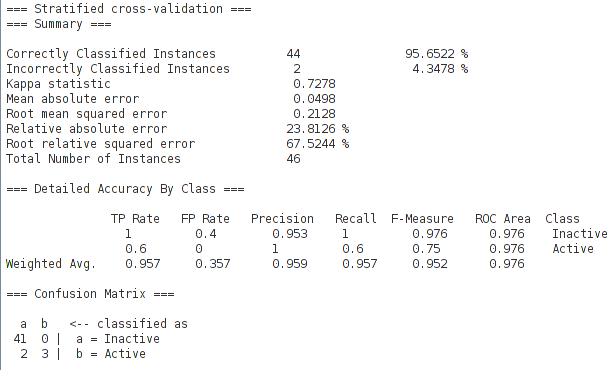
\includegraphics[scale=0.4]{figs/exp1-10CV}}\\
    \subfigure[NaiveBayes]{\label{fig:b1}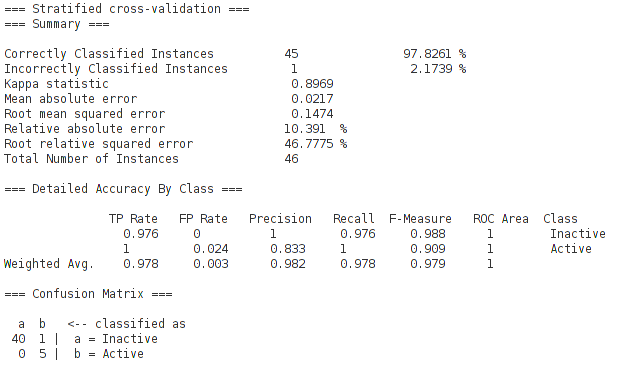
\includegraphics[scale=0.4]{figs/exp1-NB-10CV}} \\
    \subfigure[SVM]{\label{fig:c1}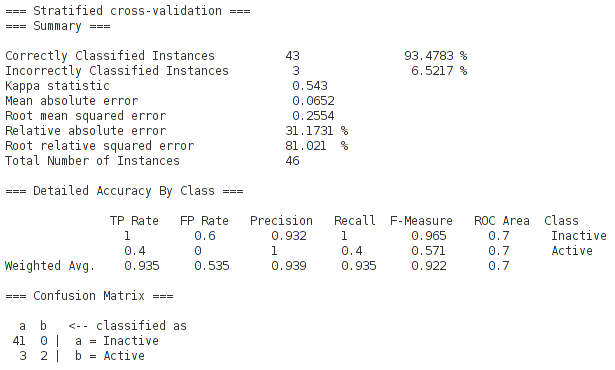
\includegraphics[scale=0.4]{figs/exp1-SVM-10CV}}\\
    \subfigure[J48 Decision Tree]{\label{fig:d1}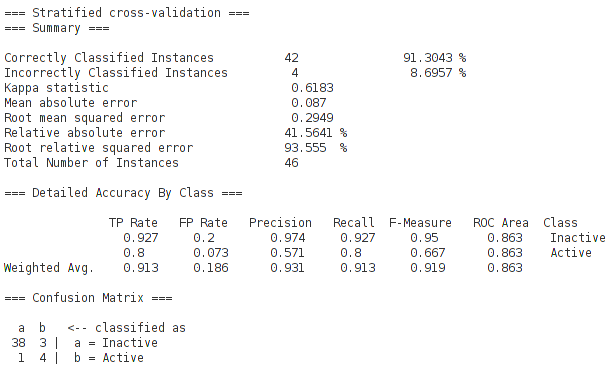
\includegraphics[scale=0.4]{figs/exp1-J48-10CV}}
  \end{center}
  \caption{Stats after running 10 Fold CV}
  \label{fig:stats1}
\end{figure}
\end{comment}
\newpage


\section{Experiment II}
In this experiment, I am going to try and do TL at assay level. Meaning I will use Active/Inactive labelled datasets from the eve data (assays TS3,4,5,6,7)
\subsection{The Data}
\begin{itemize}
\item For the $Source Dataset$, I have used TS3 (1346 instances (4 Active) -- file TS3-Labeled.arff)
\item I have randomly split TS5 into two datasets:
\begin{itemize}
\item $Target Dataset$ ... 278 instances (3 Active) -- file TS5-Labeled-Target.arff
\item $Test Dataset$ ... 1116 instances (5 Active) -- file TS5-Labeled-Test.arff
\end{itemize}
\end{itemize}  

\subsection{Experimental Setup}
Exactly the same as Experiment I

\subsection{Experimental Stat Results 1}
In this experiment I did 10 fold cross validation using the target dataset only (built models using the target dataset only and used it for the validation)
\begin{small}
\begin{center}
    \begin{tabular}{ | l | l | l | l | l | l | l | l | l | l | l | l | l |}
    \hline
      & corr & incorr  & auc & kap & mae & rmse & rae & rrse & prec & rec & fm & err rate\\ \hline
      TL  & 99.64\% & 0.35\% & 0.68 & 0.79 & 0 & 0.05 & 14.34\% & 57.83\% & 1 & 0.66 & 0.8 & 0\\ \hline
      NB  & 98.2\% & 1.79\% & 0.67 & 0.43 & 0.01 & 0.13 & 76.73\% & 130.29\% & 0.33 & 0.66 & 0.44 & 0.01\\ \hline
      J48 & 98.56\% & 1.43\% & 0.66 & 0.32 & 0.01 & 0.12 & 61.86\% & 117.27\% & 0.33 & 0.33 & 0.33 & 0.01\\ \hline
      SMO & 98.56\% & 1.43\% & 0.66 & 0.32 & 0.01 & 0.11 & 57.1\% & 115.67\% & 0.33 & 0.33 & 0.33 & 0.01\\ \hline
      IBk & 98.92\% & 1.07\% & 0.86 & 0 & 0.01 & 0.09 & 48.77\% & 89.55\% & 0 & 0 & 0 & 0.01\\ \hline

    
    
    \end{tabular}       
\end{center}
\end{small}

\subsection{Experimental Stat Results 2}
In this experiment I did 10 fold cross validation using the test dataset (built models using the target dataset and used the test dataset for the validation)
\begin{small}
\begin{center}
    \begin{tabular}{ | l | l | l | l | l | l | l | l | l | l | l | l | l |}
    \hline
& corr & incorr  & auc & kap & mae & rmse & rae & rrse & prec & rec & fm & err rate\\ \hline    
TL & 99.73\% & 0.26\% & 0.99 & 0.66 & 0 & 0.04 & 26.09\% & 74.67\% & 0.75 & 0.6 & 0.66 & 0\\ \hline
NB & 98.65\% & 1.34\% & 0.99 & 0.39 & 0.01 & 0.11 & 135.78\% & 173.48\% & 0.25 & 1 & 0.4 & 0.01\\ \hline
J48 & 99.82\% & 0.17\% & 0.89 & 0.79 & 0 & 0.04 & 18.1\% & 63.34\% & 0.8 & 0.8 & 0.8 & 0\\ \hline
SMO & 99.73\% & 0.26\% & 0.79 & 0.66 & 0 & 0.05 & 27.15\% & 77.58\% & 0.75 & 0.6 & 0.66 & 0\\ \hline
IBk & 99.55\% & 0.44\% & 1 & 0 & 0 & 0.04 & 32.77\% & 61.41\% & 0 & 0 & 0 & 0\\ \hline
    
    \end{tabular}       
\end{center}
\end{small}

\subsection{Experimental Stat Results 3}
In this experiment I did validation using the test dataset (built models using the target dataset and used the test dataset for the validation)
\begin{small}
\begin{center}
    \begin{tabular}{ | l | l | l | l | l | l | l | l | l | l | l | l | l |}
    \hline
& corr & incorr  & auc & kap & mae & rmse & rae & rrse & prec & rec & fm & err rate\\ \hline    
TL & 99.73\% & 0.26\% & 0.99 & 0.57 & 0 & 0.05 & 14.43\% & 76.81\% & 1 & 0.4 & 0.57 & 0\\ \hline  
NB & 99.28\% & 0.71\% & 0.79 & 0.49 & 0 & 0.08 & 38.46\% & 125.43\% & 0.36 & 0.8 & 0.5 & 0\\ \hline
J48 & 99.55\% & 0.44\% & 0.69 & 0.44 & 0 & 0.06 & 24.03\% & 91.42\% & 0.5 & 0.4 & 0.44 & 0\\ \hline
SMO & 99.73\% & 0.26\% & 0.7 & 0.57 & 0 & 0.05 & 14.42\% & 76.81\% & 1 & 0.4 & 0.57 & 0\\ \hline
IBk & 99.55\% & 0.44\% & 0.99 & 0 & 0 & 0.04 & 23.05\% & 73.11\% & 0 & 0 & 0 & 0  \\ \hline
    
    \end{tabular}       
\end{center}
\end{small}

\subsection{Experimental Results}
After building the models as explained above, I have evaluated them using the $Test Dataset$ which is of the same domain as the $Target Dataset$. I have counted Actual vs Predicted results.\\
The following table shows how many miss-classifications each model makes:\\ 
\begin{center}
    \begin{tabular}{ | l | l | l | p{5cm} | l |}
    \hline
    TransferBoost & NaiveBayes & SVM & KNN & J48 Decision Trees \\ \hline
    3 & 8 & 3 & 5 & 5\\
    \hline
    \end{tabular}       
\end{center}

Observe that the TransferBoost model (the one that does Transfer Learning) makes less classification errors meaning it outperforms models built using the $Target Dataset$ alone.
\begin{comment}
\begin{figure}[htp]
  \begin{center}
    \subfigure[TransferBoost TL]{\label{fig:a2}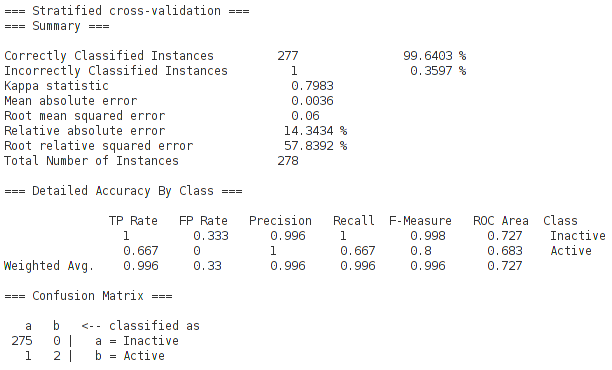
\includegraphics[scale=0.4]{figs/exp2-10CV}}\\
    \subfigure[NaiveBayes]{\label{fig:b2}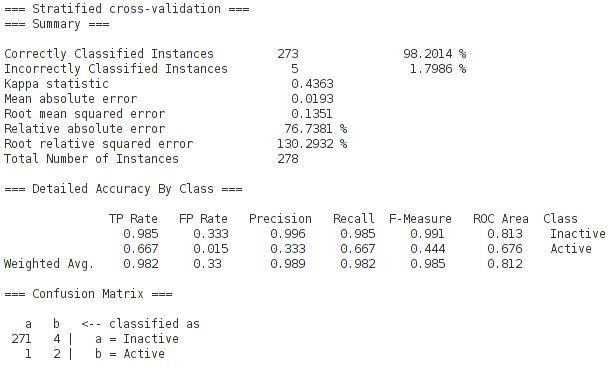
\includegraphics[scale=0.4]{figs/exp2-NB-10CV}} \\
    \subfigure[SVM]{\label{fig:c2}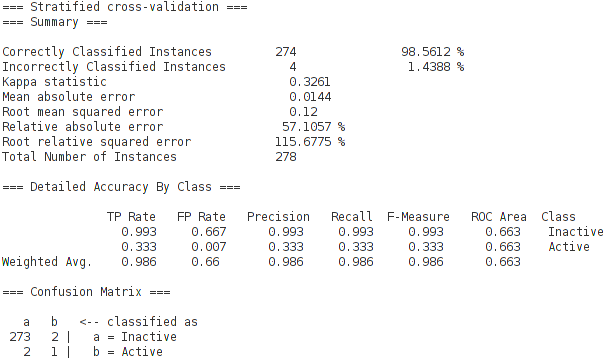
\includegraphics[scale=0.4]{figs/exp2-SVM-10CV}}\\
    \subfigure[J48 Decision Tree]{\label{fig:d2}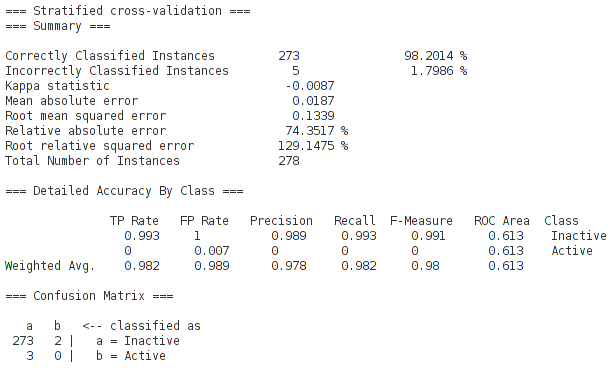
\includegraphics[scale=0.4]{figs/exp2-J48-10CV}}
  \end{center}
  \caption{Stats after running 10 Fold CV}
  \label{fig:stats2}
\end{figure}
\end{comment}
		
\end{document}
